\documentclass[lettersize,journal]{IEEEtran}
\usepackage{amsmath,amsfonts}
\usepackage{algorithmic}
\usepackage{algorithm}
\usepackage{array}
\usepackage[caption=false,font=normalsize,labelfont=sf,textfont=sf]{subfig}
\usepackage{textcomp}
\usepackage{stfloats}
\usepackage{float}
\usepackage{xurl}
\usepackage{graphicx}
\usepackage{cite}

\begin{document}

\title{F21RO - Intelligent Robotics - Coursework 2}

\author{Henri-Louis Boisvert (H00381701), Augustin Fuchs (H00380800)}

% The paper headers
\markboth{Group 13: Henri-Louis Boisvert, Augustin Fuchs}%
{Shell \MakeLowercase{\textit{et al.}}: Article presenting coursework 2}

\maketitle

\begin{abstract}
This paper describes our implementation and analysis of obstacle avoidance and line following behaviours for an e-puck robot. The goal was to get a better understanding and use of robot simulators and software tools to support the creation of intelligent controllers for robots using the bio-inspired methods covered in the course. Starting from specific environment configurations, we applied the bio-inspired algorithms to create the intelligent controllers for the e-puck robot and then we analysed the resultant robot behaviours and finally we draw conclusions from our results.
\end{abstract}

\begin{IEEEkeywords}
Behaviour Based Robotics, Evolutionary Robotics, Webots, IEEE
\end{IEEEkeywords}

\section{Introduction}
Through this assessment, we have been able to increase our understanding of the principles of Behavior-Based Robotics (BBR) and Evolutionary Robotics (ER). Furthermore, we learned to use software tools to support the creation of intelligent controllers using the techniques covered in the course. Finally, we were able to analyse the robot behaviours obtained and draw conclusions. Using the Webots simulation software, we implemented several behaviours for the e-puck mobile robot using Python for solving three different tasks. E-puck is a miniature mobile robot developed at EPFL for teaching and is based on the design of the Khepera robot. The sensors and actuators we are using are the wheel motors, the eight surrounding proximity sensors, and the three ground sensors.
\section{Task 1}
\subsection{Methods and Development Rationale}
To proceed to the obstacle avoidance approach, we had to deal with the conception of the e-puck robot. In fact, the proximity sensors which allow us to detect the obstacle cannot anticipate where the obstacle is. To know the obstacle's position and then enter an avoidance cycle, the robot must touch the obstacle throughout the avoidance. One common technique is to perform a pendulum motion to detect the obstacle's end. The robot faces the obstacle; then it starts to swing to the side where the sensors have the highest value and continues to switch between the front left and the front right sensors to keep contact with the object. 
\par
This technique is very effective on circular or rounded obstacles, the robot swings and turns around the obstacle in front of it until it finds the line again. Nonetheless, this technique can be very time consuming as the robot will move slowly, constantly alternating from one direction to another. Moreover, when the robot faces an angle or a square obstacle, it may come to the point where it is going backwards because one sensor is not facing anything at the angle. That is why we chose to design our own solution.
\par
The robot main task is to get to the end of the line regardless of the number and size of obstacles it may face.  In the robot's main routine, \texttt{sense\_and\_actuate}, if the value of the front or side proximity sensors exceeds a certain threshold, a flag: \texttt{avoid\_obs} will be set to 1. In this case, the robot will enter a new function \texttt{avoid\_the\_obstacle} that we added inside of the controller class.
The central concept of our algorithm is to avoid the obstacle by moving forward while still touching the obstacle on one side of our robot. Consequently, the e-puck will move inclined to keep contact with the obstacle thanks to one of the side sensors. When the robot approaches an angle and loses contact with the obstacle, it will rotate in the previous sense of rotation to reconnect with the obstacle. This technique is quick, simple, and even works effectively with square obstacles. If the robot loses contact with the obstacle, this program has been designed to return to the object and continue the obstacle avoidance routine.
\subsection{Obstacle avoidance routine}
The robot is following the line and is at some point facing the obstacle. The front proximity sensors are returning a high value and the program is entering into the  \texttt{avoid\_the\_obstacle} function. We designed this new routine to set the flag:  \texttt{flag\_turn}  to 1, so the e-puck is not following the line during this step. 
The second step is to get the robot off the line: while the robot is facing the obstacle in front of it, it will start turning in one direction to get the obstacle onto one side. After a specific step, the infrared sensors will not be able to detect the line anymore, and the robot will thus enter a third step which is to get back to the line. 
The e-puck will follow the outline of the obstacle and, after a certain point, will get the contact back with the line. When the robot is on the line, the last step is to align to it to continue the line following routine. This step is the fourth and last one of this obstacle avoidance process. When the robot is aligned, it must not find the object on its side, and this step will result in an avoidance routine exit, setting all the flags to 0 to continue the line following.
\subsection{Results}
Overall, this obstacle avoidance routine based on the BBR approach was quite time-consuming to implement, many parameters had to be fined tuned, and many tries were necessary to achieve this smooth avoidance. However, the results are very satisfactory and the robot can always avoid obstacles, no matter the shape. It can align and recover the line after its job is done. In all of our tests, the robot avoids the obstacle in an optimal way and turns around close to the object. To perform the task correctly, the robot must keep touching the object to get a sense of where it is because of the design of the proximity sensors, as can be seen in Figure \ref{distance_sensor}; they have an almost binary response and will not send any output if the object is not very close to the robot. Despite this, the results we obtained are satisfactory (Table \ref{task1}).

\begin{table}[H]
\begin{center}
\caption{Statistics on the time to perform task 1}
\label{task1}
\begin{tabular}{| c | c | c | c | c |}
\hline
   & First run & Second run & Third run & Average\\
\hline
Time (minutes) & 1.89 & 1.91 & 1.93 & 1.91\\
\hline
\end{tabular}
\end{center}
\end{table}

\begin{figure}[H]
\centering
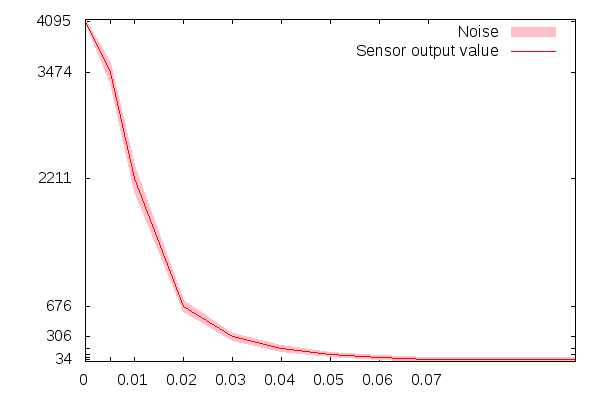
\includegraphics[width=2.5in]{distance_sensor.png}
\caption{Output given by the proximity sensors depending on the distance}
\label{distance_sensor}
\end{figure}

\section{Task 2}
The second task had for goal to discover how the supervisor is working. Implementing the obstacle avoidance required some modifications because the arena is not the same as in the first task; the behaviour of the robot also changed from line following to light following.
\subsection{Methods and Development Rationale}
The first step was to find out how to implement the obstacle avoidance routine. Entering the obstacle avoidance routine is easy because it is only required to detect the obstacle in front of us. We need to have the light detected by the front light sensors to exit this. After the robot has turned around the object, the robot will face the light. Since our obstacle avoidance routine works with the side sensors of the robot \texttt{ps2} and \texttt{ps5}, the front of our robot is kept clear to receive the light. As the two front light sensors of the robot \texttt{ls2} and \texttt{ls1} will send almost the same value if they are both seeing the light, we implemented this simple formula to exit the obstacle avoidance (\ref{light_vel}):
\begin{equation}
\label{light_vel}
f = \frac{max(ls_1,ls_2)\cdot 0.01}{min(ls_1,ls_2)\cdot 0.01}
\end{equation}
If the result of this formula is greater than or equal to 1, both sensors will be returning the same value; this value can be either their max or their low. With this added to our routine, we can avoid the obstacle and find the light again.
\par
The main task is to implement the light activation routine that will determine which one of the four corner lights should be lit inside the supervisor. To perform this simple process, we used a single light node. This light is translated in every corner position to simulate a light switched on. We found that the locations of the lights in the arena are as follow : x = 0.45 and z = 0.45, multiplied by 1 or -1 to have the all four corners. The light directions are x = 1 and z = 1, following the opposite sign of the light location. With these four parameters, we can move the light within the four corners of our arena.
\par
We added our code into the while loop of the supervisor’s controller. We initialized the \texttt{flag\_light} at -1. This flag can take a value between 0 and 3, representing the four corners of our arena. We created a list that contained all four values and made a random choice between those. After that, we got the corresponding light coordinates to set the location and direction fields with their correct vectors.
\subsection{Results}
The new supervisor light function, when combined to the obstacle avoidance does an outstanding job. After the timeout, every 60 sec, the light position will change and the robot will restart from the centre, avoiding all the obstacles it could encounter in its path.
\par
To make this task even more polished, we decided to add a condition in our light position choice step (when the light is switched on in the s
supervisor). This condition is that the light switched on at step n cannot be the same as the one at step n-1. We coded this function to avoid repeating the same step several times in a row in our simulation.
\par
In the end, we obtained very satisfactory results (Table \ref{task2}).

\begin{table}[H]
\begin{center}
\caption{Statistics on the time to perform task 2}
\label{task2}
\begin{tabular}{| c | c | c | c | c |}
\hline
   & First run & Second run & Third run & Average\\[.1em]
\hline
Time (minutes) & 1.03 & 1.08 & 1.01 & 1.04\\[.1em]
\hline
\end{tabular}
\end{center}
\end{table}

\section{Task 3}

\subsection{Methods and Development Rationale}
The third task required us to evolve a robot controller to control a single e-puck robot on the given race circuit using an Evolutionary Robotics approach. The robot should be able to follow the line on the ground at all times and at the same time avoid the obstacles while racing to finish the circuit as fast as possible. When facing an obstacle, the robot should go around it until it finds the line again.
\par
Implementing the ER approach required us to have a precise idea of the range of the sensors used by the e-puck robot to navigate. The implementation was done by analysing in Python the sensors data produced during a complete simulation. This data analysis helped us in order to normalise the sensors values. The results are satisfactory and show a wide range, with two "spikes" showing that the data returned by the sensors is not far from binary: the sensors either detect the line or not (same for the obstacles), which can be seen in Figures \ref{allSensors} and \ref{irSensors}. Normalising the sensor values has an advantage over reducing the sensors range: this gives us better results in the following functions because the lowest value will be 0, and the highest value will be 1. As the sensors values are Gaussian distributed, we took the lowest value of the distribution between the two curves: this minimized the range, and the data is then normalised without any accuracy impact.
The values obtained by this method are shown in Table \ref{tab1}:

\begin{table}[H]
\begin{center}
\caption{Sensors maximum and minimum values for normalisation}
\label{tab1}
\begin{tabular}{| c | c | c |}
\hline
 Sensor & minimum values & maximum values\\[.1em]
\hline
IR sensors & 345 & 620\\[.1em]
\hline
PS sensors & 90 & 150\\[.1em]
\hline 
\end{tabular}
\end{center}
\end{table}

\par
We then looked at the multi-layer perceptron network model used by the robot controller to make decisions. The input layer consists of seven neurons, which correspond to the four proximity sensors and three ground sensors that we will be using, and the output layer consists of two neurons outputting the left and right wheel speeds. Because there is no algorithmic way to determine the optimal structure of the MLP, we experimented with different numbers of hidden layers and different numbers of neurons for each layer. We varied the number of hidden layers from one to four and the number of neurons between one and ten, and found that three hidden layers with each ten neurons is good architecture. The activation function that we selected according to the literature is the hyperbolic tangent function.

\par
Then the main challenge was to determine the several fitness functions required to implement the ER algorithm. We experimented with different fitness functions from the broader literature \cite{ref1} \cite{ref2}.
\par
The fitness functions that we used are behavioural \cite{ref4}: those are task-specific functions that quantify some aspects of what the robot is doing and how it is doing it. This type of function will generally include some sub-functions or constants that are then combined into either a weighted sum or a product. These sub-functions and constants are intended to measure simple action-response behaviours or other events and features local to the robot. Those are referred to as behavioural terms, and they measure an aspect of how the robot is acting (behaving) but not what it has accomplished. Thus, the fitness we used only refers to the values of the sensors and cannot be based on the total distance travelled by the robot for example.
\par
The attribute that makes fitness functions behavioural is that they are made up only of values or constants that are selecting behavioural features for a presupposed solution to a given task. For example, in our case, we wanted to evolve the e-puck robot to move around the circuit and avoid the obstacles, so we included a term in the fitness function that will be maximized if the e-puck robot turns when its forward sensors are activated at close range. In this case, the ER system is set up in such a way that the robot will evolve to produce a specific actuator output in response to a specific sensor input (turning when facing an obstacle). The selection occurs for a behaviour that we believe will produce the effect of obstacle avoidance, but the robots are not evolving to avoid objects specifically, they are just learning to turn when their forward sensors are activated. This process is much more specific than just selecting robots that don't collide with obstacles.
\par
Some values in a behavioural fitness function are not selective for a precise sensor/actuator relationship, but instead for a wanted control feature. For example, if we wished to evolve a robot controller that spends most of its time moving, we would have included a value in the fitness function that is maximized when a forward motion command results in a continued forward motion of the robot (if the front of the e-puck robot was in contact with an obstacle, it would not move forward regardless of the current actuator commands). This specific function is not selective for an exact sensor/actuator relationship. Other possible functions could also produce the desired control feature, for example, a term that maximizes the ratio of forward motion to forward sensor values. Thus, this type of term does not require quite as much knowledge of the specific details of the control law that has to be learned. However, in our case, we do not have access to the actual movement of the robot, and so we have to only rely on sensor/actuator relationship functions. 
\par
Several fitness functions were thus required: a fitness function for following the line, one for moving forward,  one for avoiding obstacles, and one to avoid the spinning behaviour.
We wanted to start with a simple formula for the "moving forward" fitness function, and we found an excellent example in \cite{ref8}, with $v_l$ and $v_r$ the left and right wheel speeds:
\begin{equation}
\label{forward1}
f = \frac{v_l}{M_l}+\frac{v_r}{M_r}
\end{equation}
With $M_s$ and $M_r$ the maximum speeds of the left and right wheels.
\par
For the obstacle avoidance fitness function, we took a look at \cite{ref2}.
Letting $p_i$ denote the proximity sensors values ranging from $min_{ds}$ to $max_{ds}$, $m_l$ and $m_r$ be the left and right motor speeds and $\alpha$ and $\beta$ be numeric weights, we get (\ref{obstacle1}):
\begin{equation}
\label{obstacle1}
f = \alpha (m_l+m_r-|m_l - m_r|) - \beta \sum_{i=0}^{7} p_i
\end{equation}

Other possibilities are (\ref{obstacle2}) and (\ref{obstacle3}), with $s_{ir}$ the greatest current activation level of the proximity sensors:

\begin{equation}
\label{obstacle2}
f = mean(m_l,m_r)(1- \sqrt{|m_l-m_r|})(1-s_{ir})
\end{equation}

\begin{equation}
\label{obstacle3}
f = mean(m_l,m_r)(1- (m_l-m_r)^2)(1-s_{ir})
\end{equation}

Another variant can be found in \cite{ref3}. Letting $m_l$ and $m_r$ be the left and right motor speeds, $\alpha$ be a numeric weight and $p_i$ denote the proximity sensors values, we obtain:

\begin{equation}
\label{obstacle4}
f = \alpha (|m_l-m_r|+ |m_l| + |m_r| - (m_l + m_r)) + \sum_{i=0}^{7} p_i
\end{equation}

\cite{ref7} uses the values of specific proximity sensors, with $s_{ir1}$ and $s_{ir2}$ the values of the sensors facing the wall-side of the robot, $s_{ir3}$ the value of a sensor facing the inward side and $c_1$ and $c_2$ constants:

\begin{equation}
\label{obstacle5}
f = (s_{ir1} - c_1)^2 + (s_{ir2} - c_2)^2 + s_{ir3}^2 - (v_l + v_r)^2
\end{equation}

Then we determined the fitness function for punishing the spinning behaviour (\ref{spinning}):

\begin{equation}
\label{spinning}
f = 1 - \sqrt{\displaystyle\left\lvert \frac{m_l}{S}-\frac{m_r}{S} \right\rvert}
\end{equation}
With $S$ the maximum speed of the wheels.
Finally, the fitness function to reward the robot for following the line was implemented as follows (\ref{line}):

\begin{equation}
\label{line}
f = \begin{cases} 0 & \mbox{if $n_{activated sensors} = 0$} \\ c & \mbox{if $n_{activated sensors} = 1$} \\ 2c & \mbox{if $n_{activated sensors} = 2$} \\ 3c & \mbox{if $n_{activated sensors} = 3$}
        \end{cases}
\end{equation}
    With $c$ a constant and $n_{activated sensors}$ increasing by one for each sensor that returns a value below the threshold $t = 500$ determined from the values of Fig \ref{groundSensors}.
    
After some testing, we tried (\ref{line2}) as an alternative:
\begin{equation}
\label{line2}
f = 1 - \sqrt{\frac{\sum_{i=0}^{2} g_i}{3 M_{gs}}}
\end{equation}
with $M_{gs}$ the maximum value that can be returned by the ground sensors and $g_i$ the values returned by the ground sensors. This function is more detailed than (\ref{line}) that can only return four different values. This way, we can reward the system more precisely and get a better line-following behaviour; the function will return greater values for smaller values returned by the ground sensors, and that is the behaviour we want.
\par
We experimented with several ways to reward and punish the system: punishing hitting obstacles if the maximum value returned by the proximity sensors is above the obstacle threshold, punishing oscillatory movements when the algebraic difference between the signed speed values of the wheels is more significant than a certain threshold, punishing standing still when both wheel speeds are equal to zero and rewarding fast speed if both of the wheel speeds are greater than a certain threshold.
\par 
In the end, we decided to write our own functions, normalising the values used by the collision and the line following fitness functions (\ref{linef}, \ref{forwardf}, \ref{collisionf}, \ref{spinningf}):

\begin{equation}
\label{linef}
    lineFit = 1- \sqrt{\dfrac{\sum_{i=0}^{2} g_i}{3}}
\end{equation}

\begin{equation}
\label{forwardf}
fwdFit = \begin{cases} min(m_l,m_r) & \mbox{if $max(m_l,m_r) = 0$} \\[1em] \dfrac{min(m_l,m_r)}{|max(m_l,m_r)|} & \mbox{if $max(m_l,m_r) \neq 0$}
        \end{cases}
\end{equation}

\begin{equation}
\label{collisionf}
    collisionFit = 1 - \sqrt{\frac{max(p_i)-min\_ds}{max\_ds - min\_ds}}
\end{equation}

With $p_i$ the values returned by the proximity sensors and $min_ds$ and $max_ds$ the minimum and maximum values that can be returned by those sensors.

\begin{equation}
\label{spinningf}
    spinningFit = \frac{2^{|m_l-m_r|}}{2^{2\cdot S}}
\end{equation}
With $S$ the maximum possible speed of the wheels.
\par
Those functions were carefully designed to give the evolutionary algorithm as much information as possible, using exponents and square roots to emphasize the good fitness values and make them stand out during the process.
\begin{figure}[H]
\centering
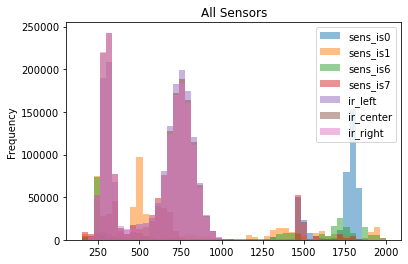
\includegraphics[width=2.5in]{allSensors.png}
\caption{Frequency of response of all sensors depending on the value}
\label{allSensors}
\end{figure}

\begin{figure}[H]
\centering
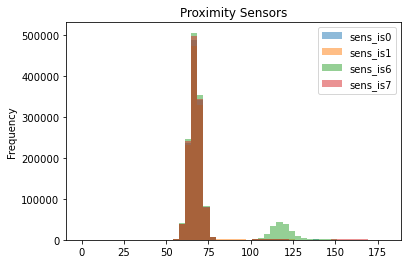
\includegraphics[width=2.5in]{proximitySensors.png}
\caption{Frequency of response of proximity sensors depending on the value}
\label{irSensors}
\end{figure}

\begin{figure}[H]
\centering
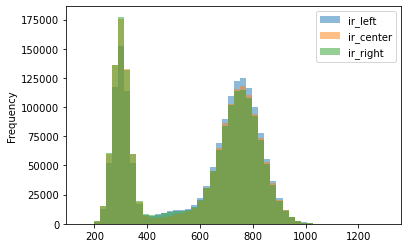
\includegraphics[width=2.5in]{irSensors.png}
\caption{Frequency of response of ground sensors depending on the value}
\label{groundSensors}
\end{figure}

The following parameters were used in the final simulation:
\begin{itemize}
    \item Mutation probability: 45\%
    \item Mutation deviation: 30\%
    \item Fitness function:
        \begin{equation}
    \label{finalFitness}
    f = forwardFit \cdot spinFit \cdot collisionFit \cdot lineFit
    \end{equation}
    With :
       \begin{equation*}
       f = \begin{cases} forwardFit = \dfrac{min(m_l,m_r)}{|max(m_l,m_r)|}
 \\[1em] spinFit = \dfrac{2^{|m_l-m_r|}}{2^{2S}} \\[1em] collisionFit = 1 - \sqrt{\dfrac{max(p_i)-min\_ds}{max\_ds - min\_ds}} \\[1em] lineFit = 1- \sqrt{\dfrac{\sum_{i=0}^{2} g_i}{3}}
        \end{cases}
        \end{equation*}
    
    With $m_l$ and $m_r$ the speeds of the left and right wheels, $S$ the maximum speed of the left and right wheels, $p_i$ the values returned by the proximity sensors, $g_i$ the values returned by the ground sensors, $max_ds$ and $min_ds$ the maximum and minimal values that can be returned by the proximity sensors and for the forward fitness, $max(m_l,m_r)$ is defined as above.

    \item Elite part: 10\%
    \item Population: 30
    \item Generations: 100
    \item Activation function: tanh
    \item Number of hidden layers in the neural network: 3
    \item Number of neurons in each hidden layer: 10
\end{itemize}
The Neuron Network architecture that we chose has the following structure (Figure \ref{nn}):

\begin{figure}[H]
\centering
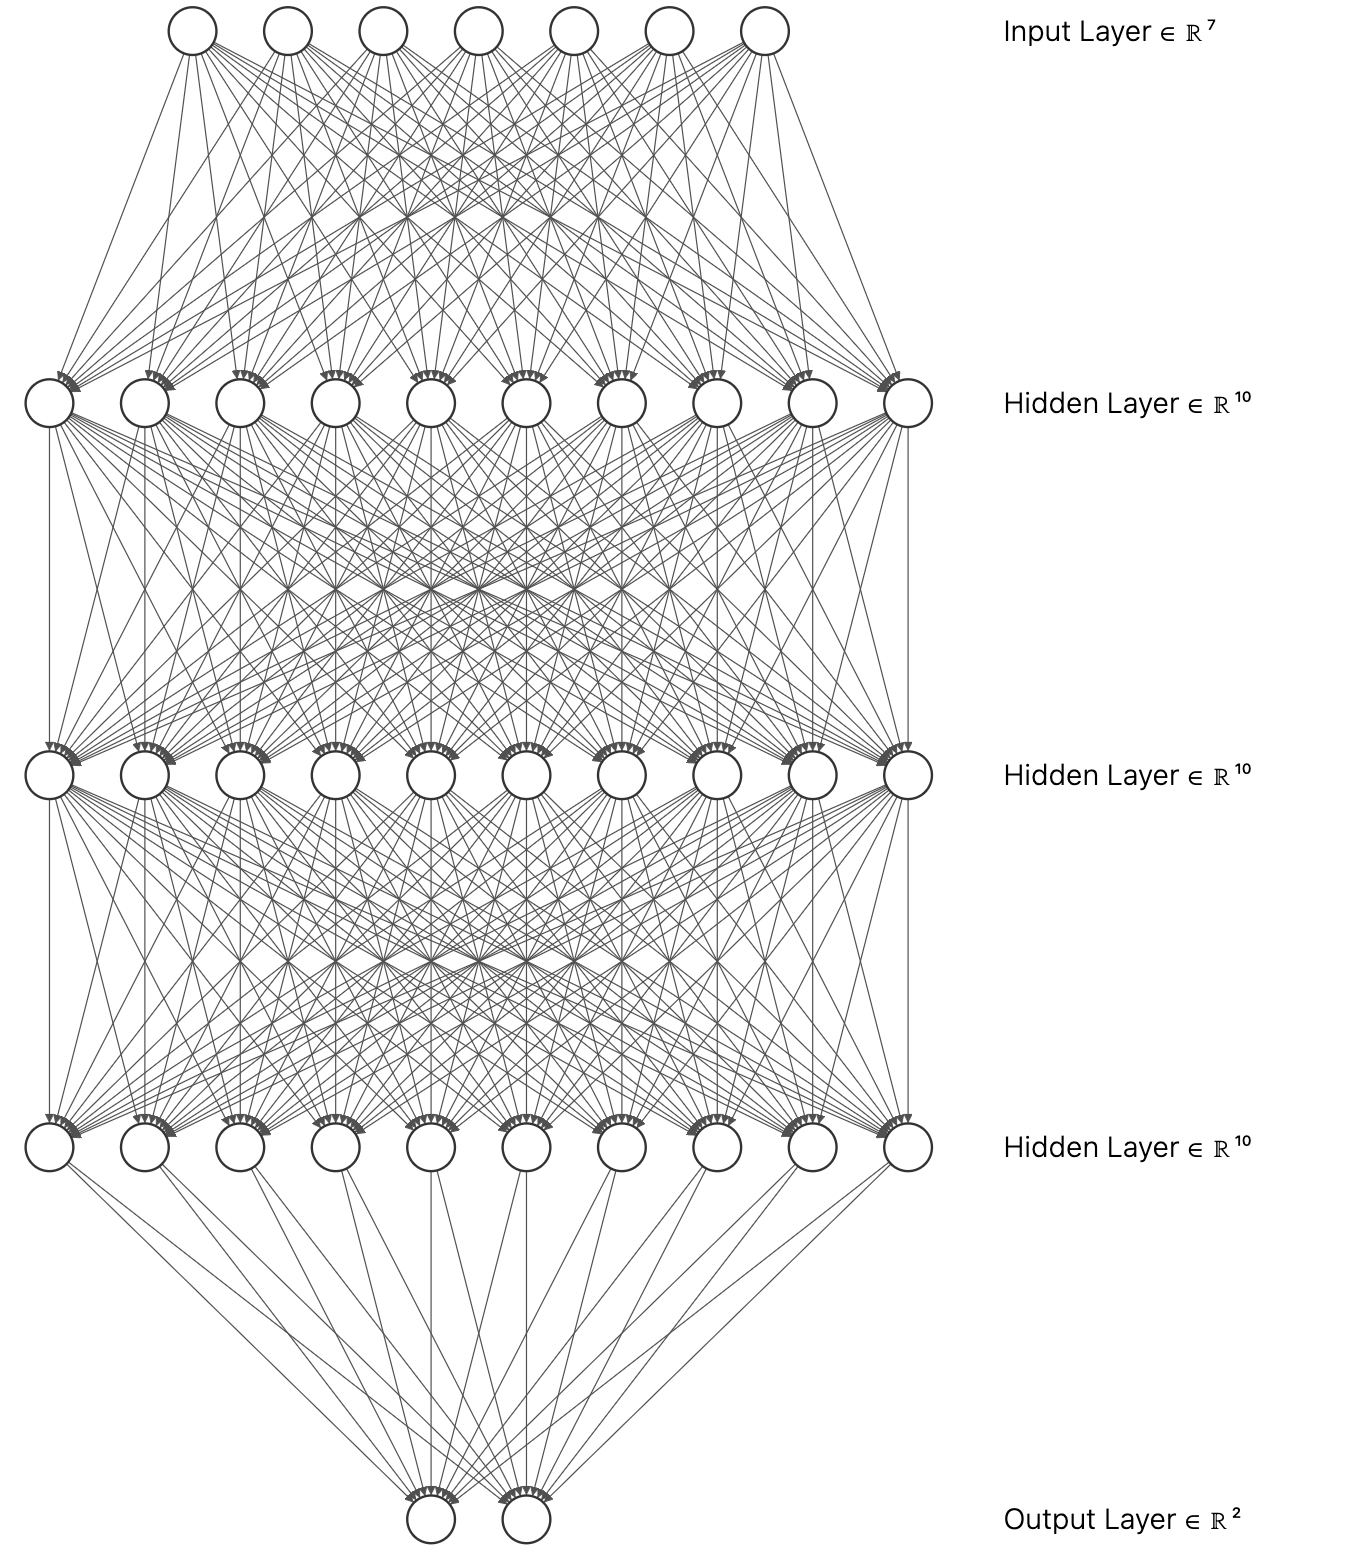
\includegraphics[width=3.64in]{nn.png}
\caption{Shape of the final Neural Network}
\label{nn}
\end{figure}


\subsection{Results}

\begin{figure}[H]
\centering
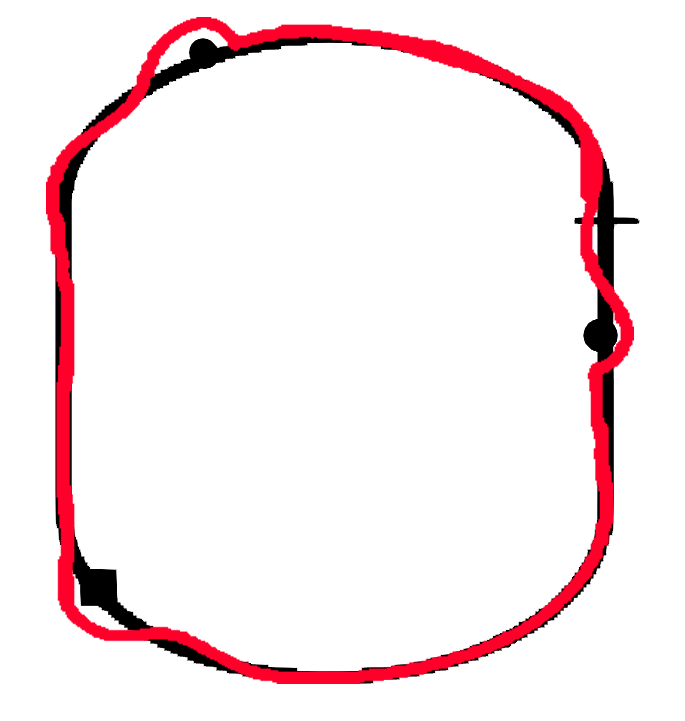
\includegraphics[width=3.5in]{path_last.png}
\caption{E-puck robot path after 100 generations}
\label{robot_path}
\end{figure}

The results we obtained are quite satisfying (Figure \ref{robot_path}). The robot can perform the task almost flawlessly and well within the expected time (see Table \ref{tab2}). The trajectory is quite impressive; the robot can easily switch between the line following and obstacle avoiding behaviours. The line following could still be slightly improved when the robot is recovering the line after avoiding an obstacle, but our implementation seems efficient.
\par
Furthermore, the equations we made regarding the different fitness functions were very reliable. In only a few generations, the robot was able to achieve the desired task. As can be noticed on the graph (Figure \ref{fitness_values}) the fitness values converge to the final fitness after a few generations. Because we decided to put a high crossover rate value, the robot tried a lot of different approaches during the training, resulting in the negative fitness values that can be seen on the graph. All in all, after only 20 to 30 generations, we obtained our maximum fitness value and the robot was able to perform its best trajectory.

\begin{table}[H]
\begin{center}
\caption{Statistics on the time to perform task 3}
\label{tab2}
\begin{tabular}{| c | c | c | c | c |}
\hline
   & First run & Second run & Third run & Average\\[.1em]
\hline
Time (minutes) & 1.00 & 1.05 & 1.15 & 1.10\\[.1em]
\hline
\end{tabular}
\end{center}
\end{table}

\begin{figure}[H]
\centering
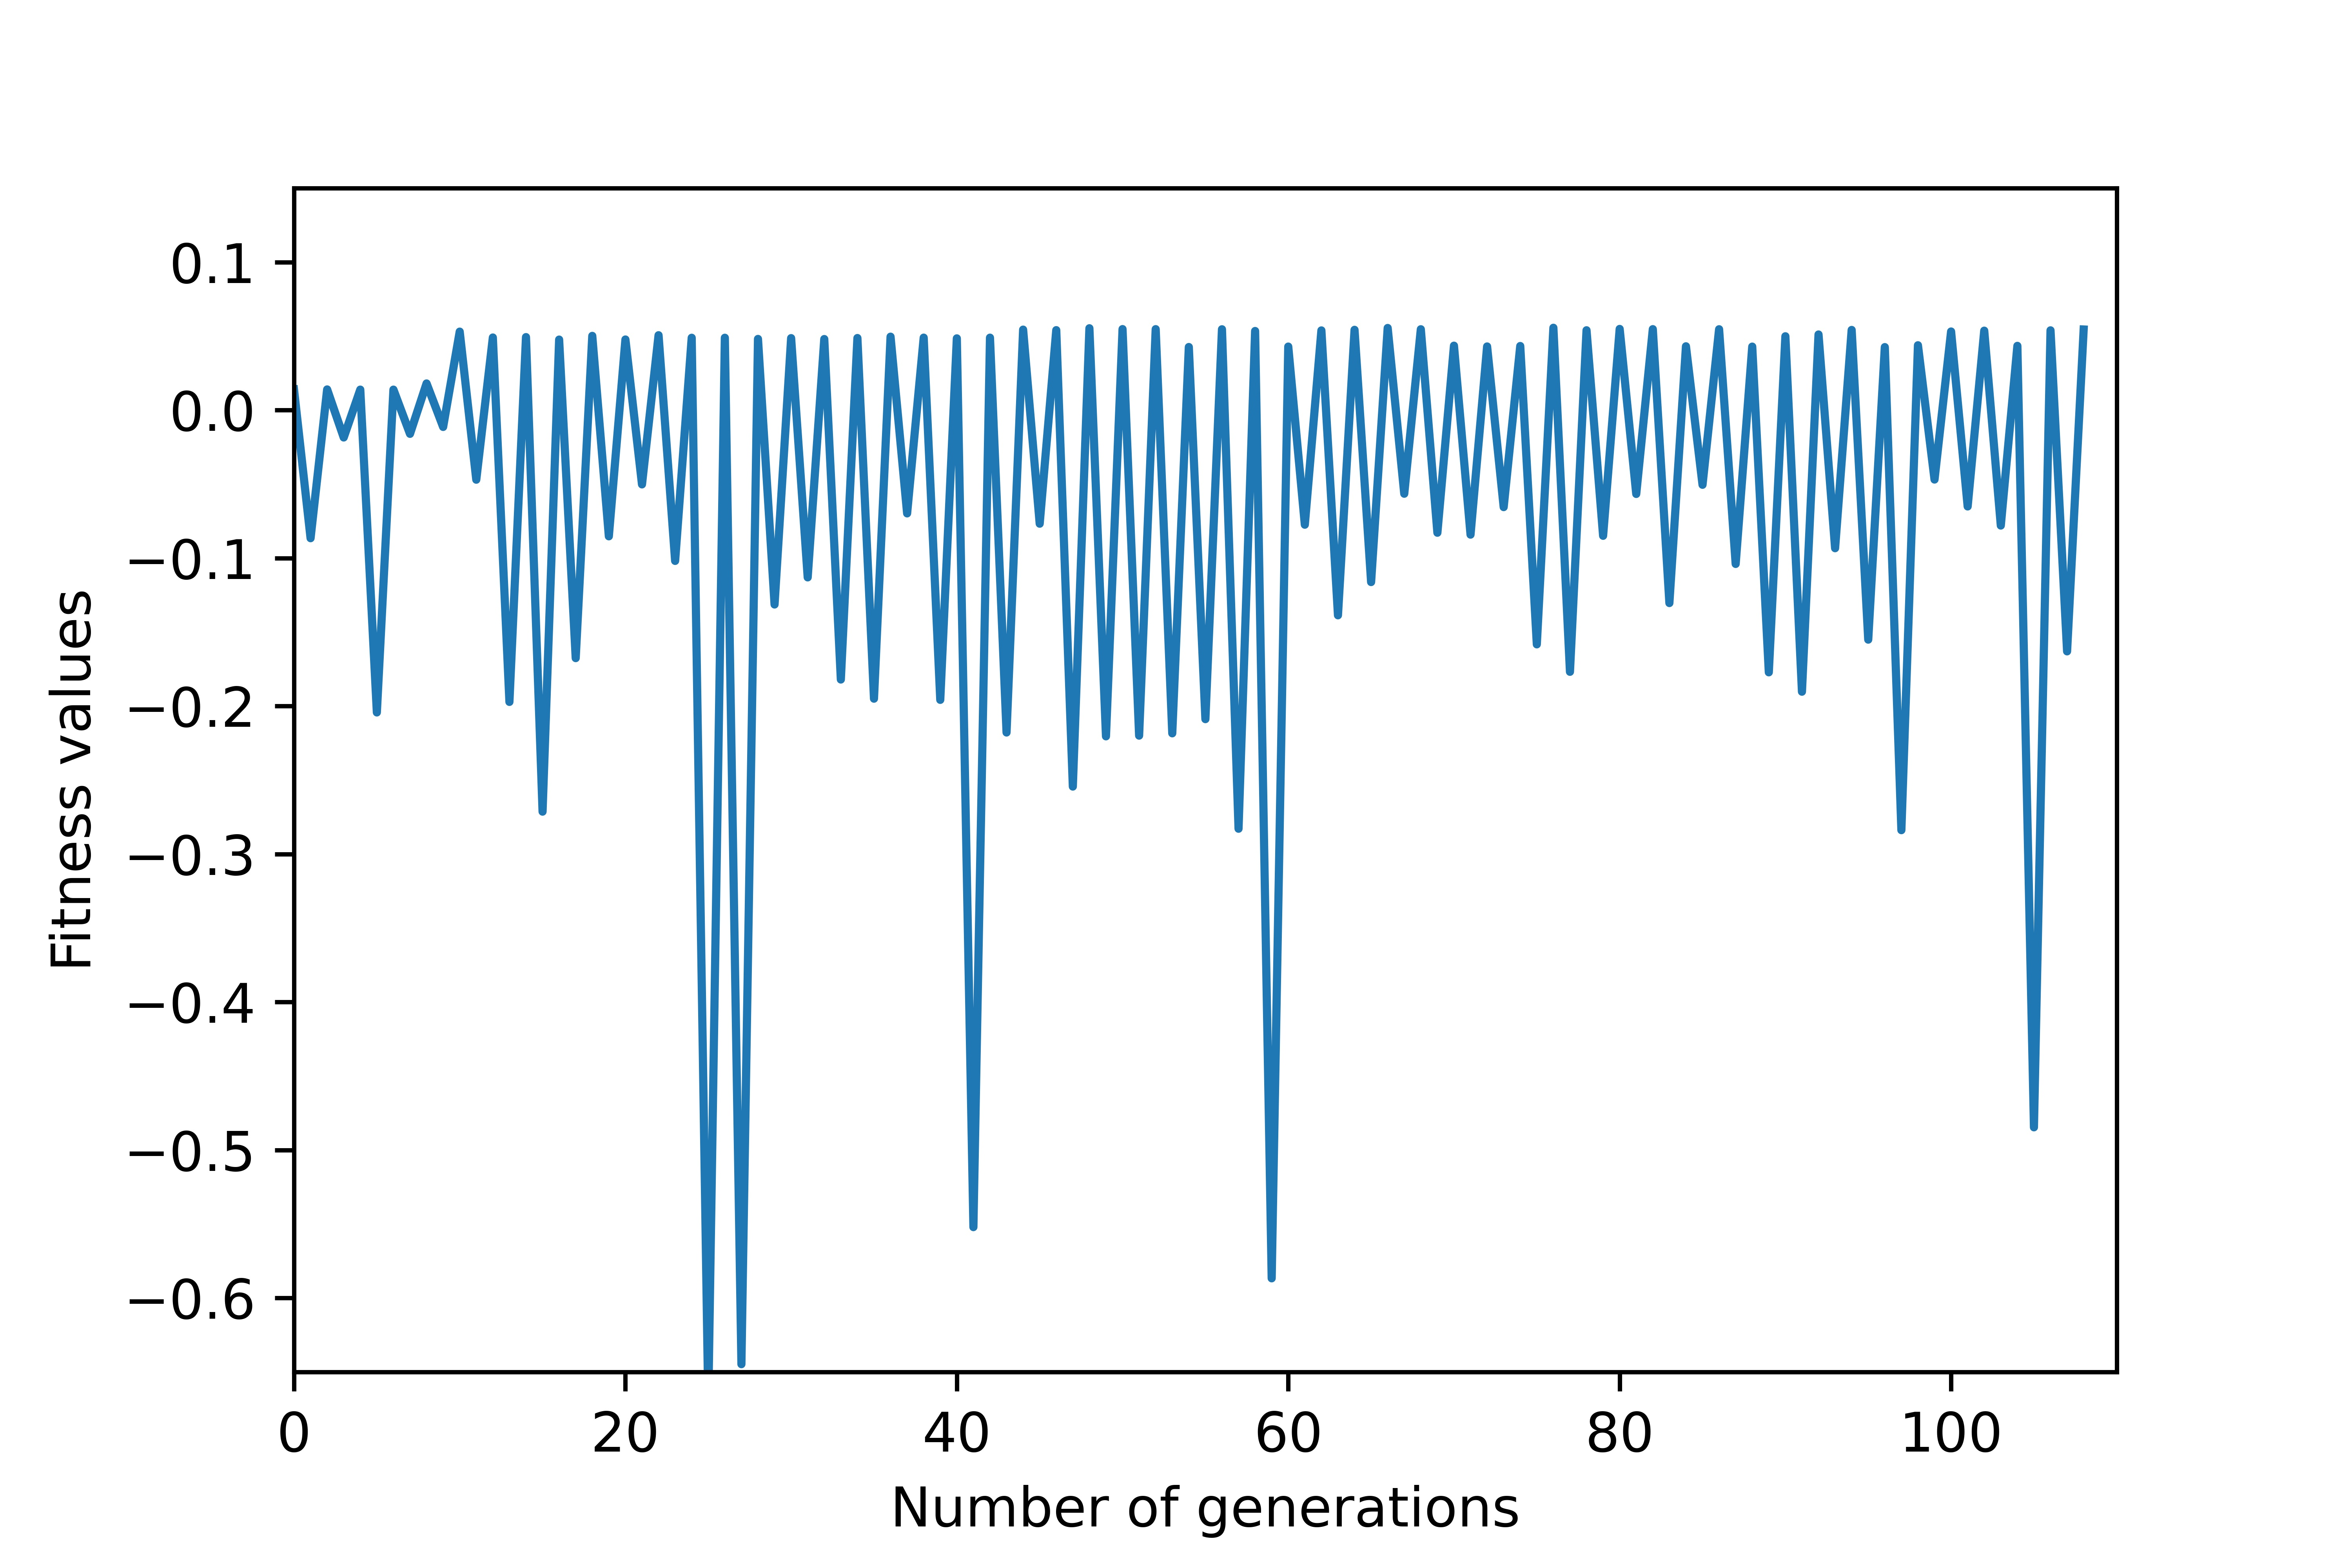
\includegraphics[width=3in]{fitness.jpg}
\caption{E-puck fitness function evolution within 100 generations}
\label{fitness_values}
\end{figure}


As mentioned by W. Banzhaf \emph{et al.} in \cite{ref1}, the environment plays a significant role in determining basic behaviours. The Evolutionary Robotic approach that we had to implement relies heavily on developing basic behaviours from the robot's setup. Depending on the environment, the global behaviours of the robot will create interactions between the basic behaviours. behaviours are then gradually adjusted, and the corresponding behaviours are closely looked at until the desired behaviours are obtained from the robot. There are two types of coordination mechanism implementation: either competitive or cooperative. The competitive method make the output depend on only one behavior, whereas for the cooperative method, the output may be depending on varied behaviours with different strengths. However, it is not clear how a specific desired behaviour should be decomposed and it is not straightforward to do this decomposition manually.
\par
The main problem we are facing is that during training, we reach a point when the fitness keeps increasing but the behaviour of the robot because less and less desirable. This means that the fitness functions we implemented do not correspond perfectly to the desired behaviours.
\subsection{Further Implementation and Improvements}
Even if we are delighted with the results we obtain with this genetic algorithm, some point still must be improved. We found the spinning fitness function and the forward fitness equation the hardest to compute. Our robot does not turn quickly because this is very costly for both forward and spinning fitness. Even if it is nothing compared to the result, the robot still hurt for a few moments the obstacle before turning.
\par
Besides, even if the e-puck robot achieves its task with very satisfying results, It is still doing undesired movements. The robot sometimes randomly turns around the last circular obstacle once or twice and continues the race, whereas sometimes it does a perfect turn. After several tries also the robot was turning right in the last obstacle, which is not the ideal trajectory. These results mean that even if our fitness functions are efficient, they are not perfect, and we can still improve them.
\par
Also, one of the main difficulties we encountered with the algorithm was to fine-tune the four fitness functions from scratch: the main problem is always designing one fitness function which does not interfere with the others. For example, the spinning fitness and the forward fitness are linked to each other because they both use the wheel velocities as variables. Therefore, it is sometimes very tricky to make them independent and not interfere with each other.
\par
As the goal of the forward fitness is to make the robot not being static or not going backwards, and the goal of the spinning fitness is to avoid a big difference between the left velocity and right velocity, we could also build a single function for this two. This could save us time for the fine tuning because there would be fewer variables.
\par
One last idea would be to make a general function with all the parameters rather than four small functions multiplying each other. With this solution, it will be probably easier to fine-tune all the parameters because they are interacting with each other only in one equation.


\section{Conclusion}

We have compared several approaches and tied different techniques throughout all this coursework. Building a BBR obstacle avoidance in task one was challenging, but it was entirely satisfactory. The robot can avoid obstacles of any shape without any difficulty and find the path again. To achieve that, we spent a lot of time fine-tuning every parameter and changing functions to make the program as efficient as possible.
\par 
We had to implement our function into the code already given during the ER approach. We tried many different combinations of fitness functions; we started by writing functions once at a time, and saw what append in the simulation. However, at this point, we saw that those functions were sometimes in conflict, but on the whole, every equation we did works, even though it took a lot of time to fine-tune. We are now confident in saying that we now understand the ER approach quite well, as our results can prove.
\par
There are many differences between BBR and ER approaches. On the one hand, we can say that the BBR approach is closer to the linear programming process that we are more familiar with, using lots of logical operators, whereas the ER approach uses a more mathematical system. However, both of these methods are time-consuming because we need to find good parameters and perform a lot of tests to make it work.  Finally, we conclude this coursework by saying that the BBR approach is efficient in terms of short tasks or single tasks, specifically in task 1. Thanks to this coursework, the both of us discovered the ER approach as a very new and different way of programming. This process revealed itself to be surprisingly efficient, with only a short amount of time to step up. However, this method was still time-consuming in terms of fine-tuning the fitness functions, but its power revealed a real advantage in multitasking projects.

\par
To conclude, we have faced several challenges during this coursework. Firstly, we had to determine the characteristics of the robot's sensors in this particular setup. This was tricky as some characteristics like the value returned by the proximity sensors seemed to change depending on whether the robot was facing an obstacle on the track or one of the walls. Then, another challenge was trying to account for the black line next to the walls of the arena, which artificially increased the fitness of some undesirable behaviours. We also had to face the fact that training the algorithm is highly resource-intensive and required us to run the simulation on a dedicated computer for more than 24 hours. Because of that, fine-tuning the numerous parameters of the simulation was extremely time-consuming. Furthermore, we had trouble determining the fitness function most appropriate for our particular environment because of the limited capabilities of the sensors and our limited computing power.
\par
We finally considered ways to improve our results \cite{ref9}. One of the solutions would have been to address the bootstrap problem: it is recognized as one of the main challenges of ER. If all the individuals from the first randomly generated population perform poorly, the evolutionary algorithm won't be able to generate any good solution. 
One solution to this would be to use a behavioural diversity method. J-B Mouret and S. Doncieux give in \cite{ref9} the process, starting from computing the distance between the genotypes of individuals (the weights of the neural network), then use this distance to modulate the fitness to promote new behaviours. However, this method needs the position of individuals to assess the distances between the genotypes, and that's impossible in our case because we are using only the sensors and the speed of the motors. Furthermore, this method would have made the process even more time consuming.
Another way to improve our results would have been to use a neural network with more layers and neurons, however this would also have made the process even more time-consuming.
\begin{thebibliography}{1}
\bibliographystyle{IEEEtran}

\bibitem{ref1}
W. Banzhaf \emph{et al.}, {\it{Genetic Programming: An Introduction on the Automatic Evolution of computer programs and its Applications, }}1998 [Online]. Available: \url{https://doc.lagout.org/science/Artificial Intelligence/Evolutionary computation/Genetic Programming An Introduction  On the Automatic Evolution of Computer Programs and its Applications - Morgan Kaufmann.pdf}

\bibitem{ref2}
W. Banzhaf, P. Nordin, {\it{Real Time Control of a Khepera Robot using Genetic Programming, }}1997 [Online]. Available: \url{https://www.cs.cmu.edu/~motionplanning/papers/sbp_papers/integrated1/khepera_genetic_1.pdf}

\bibitem{ref3}
W. Banzhaf, P. Nordin, M. Brameier, {\it{Evolution of a World Model for a Miniature Robot using Genetic Programming, }}1998 [Online]. Available: \url{http://gpbib.cs.ucl.ac.uk/cache/cache/.hidden_13-jun_567362840/http___citeseer.ist.psu.edu_cache_papers_cs_598_http_zSzzSzls11-www.informatik.uni-dortmund.dezSzpeoplezSzbanzhafzSzrobot32.pdf_nordin98evolution.pdf}

\bibitem{ref4}
A. Nelson \emph{et al.}, {\it{Fitness functions in evolutionary robotics: A survey and analysis, Robotics and Autonomous Systems, }}2009 [Online]. Available: \url{https://www.researchgate.net/publication/222655309_Fitness_functions_in_evolutionary_robotics_A_survey_and_analysis}

\bibitem{ref5}
D. Floreano, F. Mondada, {\it{Evolution of homing navigation in a real mobile robot, IEEE Transactions on Systems, Man, Cybernetics Part B: Cybernetics 26 (3), }}1996, pp. 396-407

\bibitem{ref6}
H.H. Lund, O. Miglino, {\it{From simulated to real robots, in: Proceedings of IEEE International Conference on Evolutionary Computation, }}1996, pp. 362-365

\bibitem{ref7}
W. Banzhaf, P. Nordin, M. Olmer, {\it{Generating adaptive behavior using function regression within genetic programming and a real robot, in: Proceedings of the Second International Conference on Genetic Programming, San Francisco, }}1997, pp. 35-43

\bibitem{ref8}
J. Ziegler, W. Banzhaf, {\it{Evolving control metabolisms for a robot, Artificial Life 7 (2), }}2001, pp. 171-190

\bibitem{ref9}
J-B. Mouret, S. Doncieux, {\it{Overcoming the bootstrap problem in evolutionary robotics using behavioral diversity. CEC'09: Proceedings of the Eleventh conference on Congress on Evolutionary Computation, }}2009, pp. 1161-1168 10.1109/C3EC.2009.4983077

\bibitem{ref10}
David E. Goldberg,{\it{ Genetic Algorithms in Search, Optimization, and Machine Learning-Addison-Wesley Professional }}1989

\end{thebibliography}
\end{document}


